\begin{figure}[H]
	\center
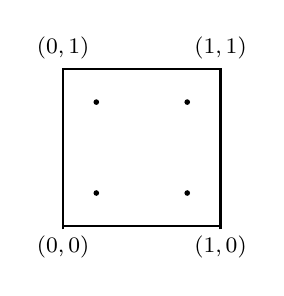
\begin{tikzpicture}[scale=2]

\draw[thick] (0,0) -- ++(1,0) -- ++(0,1) -- ++(-1,0)--cycle;
\draw[thick] (0,-0.02) -- ++(0,0.04);
\draw[thick] (1,-0.02) -- ++(0,0.04);

\filldraw (0.788675,0.211325) circle (0.4pt)
		  (0.788675,0.788675) circle (0.4pt)
	      (0.211325,0.788675) circle (0.4pt)
		  (0.211325,0.211325) circle (0.4pt);
\fill[black,font=\footnotesize] (0,0)         node[below] {$(0,0)$}
								(0,0) ++(0,1) node[above] {$(0,1)$}
								(0,0) ++(1,1) node[above] {$(1,1)$}
								(0,0) ++(1,0) node[below] {$(1,0)$};

\end{tikzpicture}

\caption{Visualisation of nodes in $\hat{\Omega}  = [0,1] \times [0,1] $}
\label{ch_quad_nodes_quadrat}

\end{figure}